% interactcadsample.tex
% v1.03 - April 2017

\documentclass[]{interact}

\usepackage{epstopdf}% To incorporate .eps illustrations using PDFLaTeX, etc.
\usepackage{subfigure}% Support for small, `sub' figures and tables
%\usepackage[nolists,tablesfirst]{endfloat}% To `separate' figures and tables from text if required

\usepackage{natbib}% Citation support using natbib.sty
\bibpunct[, ]{(}{)}{;}{a}{}{,}% Citation support using natbib.sty
\renewcommand\bibfont{\fontsize{10}{12}\selectfont}% Bibliography support using natbib.sty

\theoremstyle{plain}% Theorem-like structures provided by amsthm.sty
\newtheorem{theorem}{Theorem}[section]
\newtheorem{lemma}[theorem]{Lemma}
\newtheorem{corollary}[theorem]{Corollary}
\newtheorem{proposition}[theorem]{Proposition}

\theoremstyle{definition}
\newtheorem{definition}[theorem]{Definition}
\newtheorem{example}[theorem]{Example}

\theoremstyle{remark}
\newtheorem{remark}{Remark}
\newtheorem{notation}{Notation}

\begin{document}

\articletype{ARTICLE TEMPLATE}

\title{A Novel Optimization Framework For Optimal Sensor Deployment In Smart Buildings }

\author{
\name{Anshul Agarwal \textsuperscript{a}\thanks{CONTACT Anshul Agarwal Email: anshula@iitb.ac.in , a.anshul215@gmail.com } and Krithi Ramamritham\textsuperscript{a}}
\affil{\textsuperscript{a} Department of Computer Science and Engineering, Indian Institute of Technology (IIT) Bombay, India.}
}

\maketitle

\begin{abstract}
  Smart buildings are considered to be the new age buildings. They are expected to evolve continuously and provide intelligent solutions. This is achieved by sensing the different factors. The existing approaches overlook the problems associated with the deployment of a large number of sensors. However, this article presents a novel and holistic optimal sensor deployment method -- optimization framework for sensing different factors to make buildings smarter. It describes how intelligently using the existing information can lead to a reduction in sensors. The method is compared with the baseline approach which deploys sensors at all the locations where they should be sensed. This optimization framework has been compared with the baseline approach for an existing building. The results indicate that the newly developed optimization framework requires 72.92\% less sensors as compared to the baseline approach. This feature makes it an impressive proposition and results in much less in e-waste generation. 
\end{abstract}

\begin{keywords}
Smart Buildings; Sensor Deployment; Optimization Framework; Baseline Approach; Sensor Reduction;
\end{keywords}

\section{Introduction}

Internet of Things (IoT) and Cyber-Physical Systems (CPS) are the two very commonly heard terms nowadays. Due to the advent of these technologies, buildings have evolved from being intelligent to becoming smarter. A smart building is expected to fulfill tasks like monitoring the health of appliances, provide thermal comfort to the users (Reena et al. 2018), track occupants in the building, and optimize and reduce the wastage of energy (Karmakar et al. 2018). However, fulfilling these tasks requires sensing of factors such as energy consumption, occupancy and type of appliances that are switched ON. Therefore, it is important to deploy sensors in the building to sense these factors of interest (Agarwal et al. 2016a). There exist various techniques for placement of sensors in the buildings to sense different factors (Ref. …??..). However, these techniques do not consider the issues related to the deployment of a large number of sensors, such as increased user inconvenience and capital cost of procuring, installing, maintaining and upgrading the sensors, disturbing the aesthetics of the building, incremental investment on storage and communication facilities for the sensors and threat to privacy (Hnat et al. 2011, Stankovic et al. 2014). The most worrying drawback of these techniques is the increased generation of e-waste. 
In 2016, the CEO of SoftBank Group Corporation estimated that there would be at least a trillion connected devices around the world in the next 20 years (Higginbotham, S., 2018). However, the existing techniques fail to provide effective solutions with sensor minimization as an important parameter.

In fact, rapid research in data mining, algorithms, and machine/deep learning approaches has led to efficient techniques for processing large amounts of sensor data. This encourages the approach of throwing sensors at the problem so that large amounts of data are generated and can be processed to provide smart applications and experience. 

The objective of this article is to provide an approach that reduces the number of sensors to be deployed to overcome the various issues related to the deployment of a large number of sensors in a smart building. The major contribution of this article is a novel and holistic approach to optimal sensor deployment in buildings to make it smarter by sensing the factors of interest. It uses soft sensing, which implies inferring a factor from another set of factors, as the primary tool to reduce the deployment of sensors; it defines how existing information can be intelligently used to infer the factors of interest, and thus reduce the number of sensors to be deployed. For instance, Ciftler et al. (2018) demonstrated how occupancy can be inferred in the buildings using the Wi-Fi signal information. The effectiveness of this approach is tested on a real-world problem of sensor deployment in an existent building to make it smarter and demonstrate an impressive reduction in sensors.

\section{Literature Review}

\textbf{?? to review refs ?? ??}

One of the biggest challenges in smart buildings is the storage and analysis of real-time sensor data (Zanella et al., 2014; El-Shafie et al., 2018).  Bashir et al., (2016) proposed a technique for the integration of big data analytics and IoT for effectively dealing with real-time building sensor data. Biljana et al. (2017) described a holistic framework for integrating smart home objects into a cloud-centric framework. Minoli et al. (2017) discussed the various practical challenges faced by the Internet of Things in smart buildings. Pan et al. (2015) proposed an IoT framework that used smartphone and cloud platforms for saving energy and improving the home network intelligence. Hernández-Ramos et al. (2015) proposed an ARM compliant security framework using IoT. Ghayvat et al. (2015) discussed how wellness of the home residents is monitored to determine if they are fine and extended this approach to the smart building environment. 

Weng et al. (2012) used different information to optimally plug level loads and HVACs for saving energy of the building. Magno et al. (2015) proposed a low cost, wireless, easy to install, adaptable, and smart LED lighting system to automatically adjust the intensity of light for saving energy. Basu et al. (2014) described a sensor-based intelligent lighting system for future grid-integrated buildings. A technique for optimizing energy usage and improving the thermal comfort of residents in smart buildings is discussed by Schumann et al. (2014). Yang et al. (2014) proposed an approach for learning interaction between the residents and nest learning thermostats in the building to improve energy savings and user comfort. Data-driven system to estimate personal energy footprint in real-time has been discussed by Wei et al. (2018). Shwehdi et al. (2015) presented a case study on how HVACs affect building energy consumption. Factors such as power supply and others that are important for user comfort are discussed by Au-Yong et al. (2019). Gul et al. (2015) presented a work that illustrates the relationship between occupancy and energy behavior of the building. A novel approach of using environmental and room sensors to control the installed HVACs is demonstrated by Hafeez et al. (2017). Using the resident’s feedback to maintain a comfortable temperature inside the room has been investigated by Shin et al. (2017). 

There exist multiple works that discuss inferring a factor from other sets of factors (Agarwal et al. 2016c). Using virtual sensors to abstract hard sensors for programmatically specifying high-level requirements has been described by Kabadayi et al. (2006). Using Wi-Fi signals to infer the occupancy status and information has been demonstrated by Çiftler et al. (2018), Thanayankizil et al. (2012) and Balaji et al. (2013). Occupancy prediction using CO2 based physical and statistical modeling has been investigated by Zuraimi et al. (2013). Salimi et al. (2019) proposed an adaptive probabilistic occupancy prediction model. Ekwevugbe et al. (2013) discussed a low cost and non-intrusive method for sensor network deployment to combines information such as sound level, case temperature, CO2 and motion. Learning about occupants and their sleep patterns to optimally operate HVACs has been described by Lu et al. (2010). 


\section{Methodology}

In this article, a new optimization framework has been developed for optimal sensor deployment. This optimization framework outputs the optimal number, type, and location of sensors such that required factors are sensed in the smart buildings. 


A block diagram to summarize the proposed optimization framework has been demonstrated in Figure ??. The various inputs and symbols used in the framework are described in Table ??.





\subsection{Application Area}

For the application of optimization framework, a set of rooms of KReSIT building of the Computer Science and Engineering Department, IIT Mumbai (India) was selected. The building consists of one HVAC room and two levels. Each level consists of one small and one big room as shown in Figure 2. Each big room was divided into two zones to sense different factors. A separate location for the HVAC room is denoted since it provides common cooling to all the rooms of the building and consumes a very high amount of energy. 


\subsection{Optimization Framework}

It consists of an objective function and set of constraint functions which are described as follows.

\subsubsection{Objective Function}

It is used to specify the aim of deploying minimum number of sensors in the building to sense factors.

\begin{equation}
  minimize \sum_{l \in \{L\}} \sum_{k \in \{K\}} \sum_{s \in \{s^k\}}  used(l,k,s)
\end{equation}

\subsubsection{Constriant Functions}

\noindent $\bullet$ Sensing Requirement: this constraint ensures that the final optimal sensor allocation satisfies the sensing requirement required for the smart building.

\begin{equation}
  \forall l \in \{L\} \;\; \forall k \in \{K\} \quad sensed(l,k) = tosense(l,k)
\end{equation}

\noindent $\bullet$ Sensing Rules: for sensing a factor k at a location l, the following sensing rules apply.

  Rule 1: If a sensor $s_i^k$ is deployed in l	ocation l, then the factor k is sensible in location l.

	Rule 2: If a soft sensor, that infers factor k from factors $\{k_i\}$, is deployed in location l
and factors $\{k_i\}$ are sensible in location l, then the factor k is sensible in location l.

\noindent This constraint is represented as:

\begin{equation}
  \forall l \in \{L\} \;\; \forall k \in \{K\} \quad sensed(l,k) = \max \left(
  \sum_{s \in \{s^k\}}  used(l,k,s) , 
  \prod_{j \in \{k_i\}} sensed(l,j)
  \right)
  \end{equation}

  \noindent $\bullet$ Sensing from sub-locations: A location may be composed of sub-locations or relatively small locations (Figure 2). Let the sub-locations of a location l be represented by $\{subl^l\}$. Thus, this constraint states that if a factor k that is sensible in all the sub-locations of a location l, then the factor k is also sensable at location l. For example, consider a room that consists of two zones. To sense the temperature of a room, temperature values of its sub-locations, i.e., zones are sensed using hard sensors. These values are then aggregated using a function like average to represent the temperature of the room.

  \begin{equation}
    \forall l \in \{L\} \;\; \forall k \in \{K\} \quad sensed(l,k) = \max \left(
  \sum_{s \in \{s^k\}}  used(l,k,s) , 
  \prod_{sub \in \{subl_l\}} sensed(sub,k)
  \right)
  \end{equation}

  \noindent $\bullet$ Limiting the sensors: if $limit(s_i^k)$, which represents the maximum number of sensor $s_i$ sensing factor k that can be deployed, is provided as input, then this constraint ensures that the total number of sensors of the type $s_i^k$ deployed in the optimal sensor allocation does not exceed the provided limit.

 \begin{equation}
    \forall k \in \{K\} \;\; \forall s \in \{s^k\} \quad \left(
      \sum_{l \in \{L\}} used(l,k,s)
    \right) \leq limit(s)
   \end{equation}

\section{Results And Discussion}

A smart building provides thermal comfort at optimum power consumption based on the occupancy. It can be achieved by occupant detection and appliance automation. To fulfill these tasks, four primary factors need to be sensed: power consumption, number and type of ON appliances, occupancy and temperature of the rooms.

\subsection{Inputs used for optimal sensor allocation}

\begin{itemize}
  \item Set of Locations $\{L\}$: as represented in Figure 2.
  \item Factors to Sense: power consumption, number and type of ON appliances, occupancy and temperature.
  \item Type of Sensors: used to sense the above factors as shown in Table 2.
  \item Sensing Requirement: All the factors in all the locations, except HVAC room $(L^{HR})$, should be sensed. 
\end{itemize}
  
\begin{equation}
  \forall l \in \{L \setminus L^{HR} \} \;\; \forall k \in \{K\} \quad tosense(l,k) = 1
\end{equation}

For location HVAC room $L^{HR}$, only power consumption should be sensed since the room is never occupied, and sensing other factors is not meaningful.

\begin{equation}
  \begin{split}
    tosense(L^{HR}, power) = 1 \\
    \forall k \in \{K \setminus power \} \quad tosense(L^{HR},k) = 0
  \end{split}
\end{equation}


\subsection{Output}

The optimization framework has been implemented in python library PuLP (Mitchell et. al. 2011) which is used for solving linear programs. When the various inputs (as discussed in the previous section) are given to the optimization framework, it implements the objective function Eq. (1) and constraint functions (Eq. (2) – (5)) to output the optimal sensor allocation for the application area, whose details are summarized in Table 3 and Table 4.

Observing the sensed matrix (Table 3), it can be concluded that the sensing requirement of sensing all the factors in all the locations, except HVAC room where only power consumption should be sensed, is satisfied by the optimization framework. The details of optimal sensor allocation for satisfying the sensing requirements is denoted by used matrix (Table 4) and are explained as follows. 

\begin{itemize}
  \item 1.	Since no soft sensor is available to sense temperature (Table 2), two hard sensors are used to sense the temperature in two small rooms (one for each room) and four sensors for big rooms (one for each zone). In big rooms, the temperature is sensable since temperature of the zones is sensed (Constraint C, Eq. (4)). Similarly, the temperature of levels and the building become sensable. Thus, a total of six temperature sensors are deployed.
  \item Occupancy is sensed either by placing Passive infrared (PIR) sensor or a camera in two small rooms (one for each room) and two big rooms (one for each zone). No soft sensor is used since occupancy cannot be inferred from the other factors in these locations. Using Constraint C Eq. (4), occupancy of big rooms, levels and the building becomes sensable. Therefore, a total of six PIR + camera sensors are deployed.
  \item Information of ON appliances can be inferred from occupancy and temperature using a soft sensor (Table 2). Since all the locations already sense temperature and occupancy, the number and type of ON appliances is sensed using the soft sensor (Constraint B, Eq. (3)). Therefore, no hard sensor is deployed to sense this factor.
  \item In the HVAC room, only one smart meter is placed to sense power consumption since no other factor is sensed at this location. In all the remaining locations, power consumption is inferred from number and type of ON appliances information using a soft sensor (Constraint B, Eq. (3)).
\end{itemize}

Therefore, to sense the factors in all the locations of the building, only 13 sensors are required as tabulated in Table 5.

However, the effectiveness of the proposed optimization framework is compared with baseline approach method for sensor deployment at the same application area. The baseline approach consists of deploying appropriate sensors for all the factors in all the locations where they should be sensed. For example, to sense power, ON appliances, occupancy, and temperature in all the location of the building (Figure 2), four sensors (one for each factor) is deployed in all the locations, leading to the deployment of 48 sensors as shown in Table 6.

Therefore, it can be concluded that newly developed optimization framework is highly effective technique as compared to baseline method. Because to sense the same amount of data, baseline method needs 48 sensors while the newly developed optimization method requires only 13 sensors, which is about 72.9\% saving in number of sensors to be deployed. 

This impressive reduction demonstrates how practical the proposed technique is and should be used as a primary tool for sensing factors when developing smart cities and buildings. For example, if this methodology is used for a smart city consisting of one thousand smart buildings of the same size and design (as described in the application area), it will require only thirteen thousand sensors while the baseline approach will require forty-eight thousand sensors, resulting into a net saving of thirty-five thousand sensors.

However, in the semi-smart buildings, sometimes it is required to sense only one or two parameters. For example, it may be required to sense only number of ON appliances at any one time or total power consumption of the building. Under all such scenarios, the developed optimization framework is very effective as compared to baseline approach as shown in Table 7.

It is depicted from Table 7 that for sensing the number of ON appliances only twelve sensors are required by using the baseline approach. However, only seven sensors are required using the newly developed optimization framework. Similarly, to measure the power consumption, twelve and seven smartmeters are required using the baseline approach and developed optimization framework, respectively. Therefore, the new developed optimization framework is an effective tool to reduce the number of sensors required to make buildings smarter.

\section{Conclusion}

Various factors such as power consumption, ON appliances, occupancy and temperature can be sensed using a minimum number of sensors.  This can be achieved by using the newly developed optimization framework which is an effective tool to reduce the number of sensors required to sense various factors in a smart building. This optimization framework has been compared with the baseline approach and results are found to be very encouraging. When this technique is applied to an existing building, it requires 72.92\% less sensors as compared to the baseline approach. This feature makes it an impressive proposition and leads to a large reduction in e-waste generation. Therefore, it can be concluded that if the existing information is used intelligently, it will lead to a reduction in sensors. 


% \begin{figure}
% \centering
% \subfigure[An example of an individual figure sub-caption.]{%
% \resizebox*{5cm}{!}{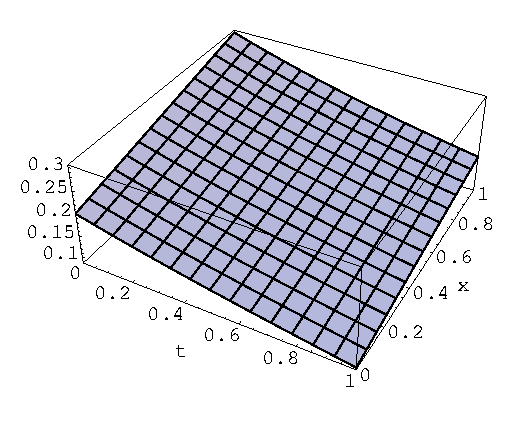
\includegraphics{graph1.eps}}}\hspace{5pt}
% \subfigure[A slightly shorter sub-caption.]{%
% \resizebox*{5cm}{!}{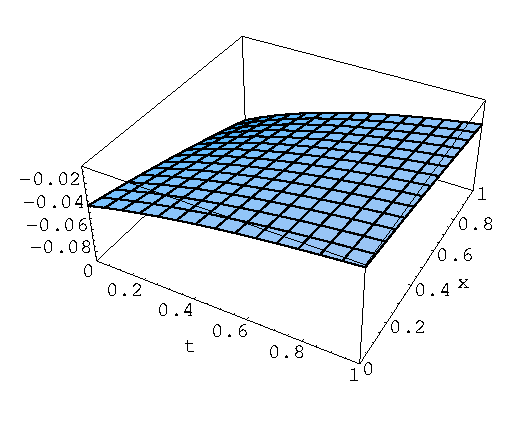
\includegraphics{graph2.eps}}}
% \caption{Example of a two-part figure with individual sub-captions
%  showing that captions are flush left and justified if greater
%  than one line of text.} \label{sample-figure}
% \end{figure}

% \begin{table}
% \tbl{Example of a table showing that its caption is as wide as
%  the table itself and justified.}
% {\begin{tabular}{lcccccc} \toprule
%  & \multicolumn{2}{l}{Type} \\ \cmidrule{2-7}
%  Class & One & Two & Three & Four & Five & Six \\ \midrule
%  Alpha\textsuperscript{a} & A1 & A2 & A3 & A4 & A5 & A6 \\
%  Beta & B2 & B2 & B3 & B4 & B5 & B6 \\
%  Gamma & C2 & C2 & C3 & C4 & C5 & C6 \\ \bottomrule
% \end{tabular}}
% \tabnote{\textsuperscript{a}This footnote shows how to include
%  footnotes to a table if required.}
% \label{sample-table}
% \end{table}


?? ?? \cite{Bro02}


\bibliographystyle{tfcad}
\bibliography{interactcadsample}

\end{document}